\documentclass{article}
\usepackage{amsmath}
\usepackage[margin=1in]{geometry}
\usepackage{amsfonts}
\usepackage{hyperref}
\usepackage{graphicx}
\usepackage{amssymb}

\begin{document}
	
	\title{Determinant}
	\author{Andy Chong Sam}
	
	\maketitle	
	
	\section{Geometric Intuition of Determinants}
	
	\par \noindent This document offers a geometric intuition of the determinant for a 2x2 and a 3x3 matrix. We start with the idea of a \textbf{square matrix} which is one that has an equal number of rows and columns. A 2x2 square matrix is therefore capable of holding two vectors each containing 2 components, and a 3x3 matrix can hold three vectors each containing 3 components.
	\newline
	\par \noindent We will show that the determinant of a 2x2 matrix is the area of the parallelogram formed by two vectors. It can also be shown that the determinant of a 3x3 matrix is the volume of a parallelepiped formed by three vectors.
\section{A 2x2 matrix}
\par \noindent To show that the determinant of a 2x2 matrix is the area of the inscribed parallelogram from figure 1 we can start by defining matrix A comprised of two generic vectors. This vector along with its determinant is shown below:
\[A=
\left(\begin{array}{@{}cc@{}}
	a_x & b_x \\ 
	a_y &  b_y \\
\end{array}\right)
\therefore det(A) = a_x b_y - b_x a_y\]
\newline
	\begin{minipage}[c]{.25\linewidth}
		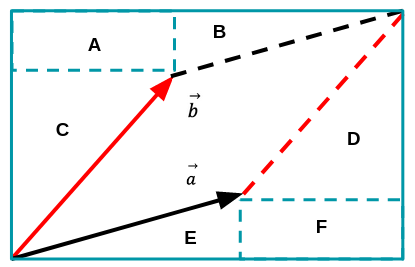
\includegraphics[width=5cm]{parallelogram2by2.png}\newline
		\begin{center}\textbf{Figure 1}\end{center}
\end{minipage}
\hspace{1.5cm}
\begin{minipage}[c]{.75\linewidth}
	\par \noindent \textbf{(Total Area)} \(= (a_x + b_x)(a_y + b_y)=a_xa_y+a_xb_y + b_xa_y+b_xb_y\)
	\par\noindent \textbf{(A \& F)} = \(b_xa_y\), \textbf{(B \& E)}=\(\frac{1}{2}a_xa_y\), \textbf{(C \& D)}=\(\frac{1}{2}b_xb_y\)
\end{minipage}
\newline
\newline
\par\noindent The area of the inscribed parallelogram will be the total rectangle area minus the sum of the named components. This result is the determinant of matrix A:
\begin{flalign*}
	a_xa_y + a_xb_y + b_xa_y + b_xb_y - 2b_xa_y - a_xa_y - b_xb_y \\
	=a_xb_y + b_xa_y - 2b_xa_y \\
	=a_xb_y - b_xa_y	
\end{flalign*}
\par \noindent In the case of a 2x2 matrix, the determinant is equivalent to the cross product of the two vectors. Since it's a scalar we can refer to this calculation as: \(|| \vec a \times \vec b  ||\).
\newpage
\section{A 3x3 matrix}
\par\noindent The determinant of a 3x3 matrix is the volume of a parallelepiped formed by three vectors. This can be conveyed through the following matrix: 
		 \[B=
\left(\begin{array}{@{}ccc@{}}
	a_x & b_x & c_x \\ 
	a_y &  b_y & c_y \\
	a_z &  b_z & c_z \\
\end{array}\right) \therefore det(B)=(a_xb_yc_z+a_zb_xc_y + a_yb_zc_x) -(a_zb_yc_x + a_xb_zc_y + a_yb_xc_z)
\]


	\begin{minipage}[c]{.25\linewidth}
	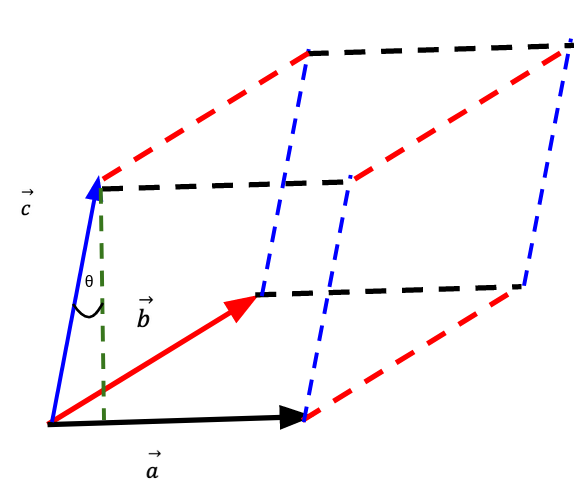
\includegraphics[width=5cm]{parallelipiped.png}\newline
	\begin{center}
		\textbf{Figure 2}
	\end{center}
\end{minipage}
\hspace{1.5cm}
\begin{minipage}[c]{.75\linewidth}
	
	\par \noindent The volume of such a figure will be its base multiplied by its height. 
	\newline
	\par \noindent \textbf{Base:} \( || \vec a \times \vec b  ||\)
	\newline
	\par \noindent \textbf{Height:} \(||\vec c||cos \theta\) 
	\newline
	\par \noindent \textbf{Volume:} \(||\vec a \times \vec b||\)  \(||c||cos \theta\)
	\newline
	\par \noindent Using the law of cosines, the volume can be rewritten to: \(  (\vec a \times \vec b)\cdot \vec c\) .
	 
\end{minipage}
\newline
\newline
\par\noindent We can now carry out the triple scalar operation which will the determinant of matrix B:
\[  (\vec a \times \vec b)\cdot \vec c=
\left(\begin{array}{@{}ccc@{}}
	a_yb_z - a_zb_y & -a_xb_z + a_zb_x & a_xb_y-a_yb_x
\end{array}\right) \cdot
\left(\begin{array}{@{}c@{}}
	c_x \\ 
	c_y \\
	c_z
\end{array}\right)  
\]

\begin{flalign*}
	c_x(a_yb_z-a_zb_y) + c_y(-a_xb_z+a_zb_x) + c_z(a_xb_y - a_yb_x)	\\
	= a_yb_zc_x - a_zb_yc_x - a_xb_zc_y + a_zb_xc_y + a_xb_yc_z - a_yb_xc_z \\
	= (a_xb_yc_z + a_zb_xc_y + a_yb_zc_x) - (a_zb_yc_x + a_xb_zc_y + a_yb_xc_z)
\end{flalign*}
\section{Determinant and Independence}
\par\noindent There are many useful properties for the determinant, but in this document we'll highlight the relationship between linear independence and the determinant. \textbf{If a set of vectors is linearly dependent, then its determinant is zero.}
\newline
\newline
\begin{minipage}[c]{.50\linewidth}
	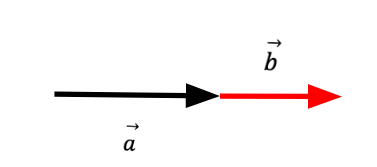
\includegraphics[height=3cm]{no-parallelo.png}
	\begin{center}\par \noindent Figure 3\end{center}
\end{minipage}
\hspace{0.75cm}
\begin{minipage}[c]{.50\linewidth}
		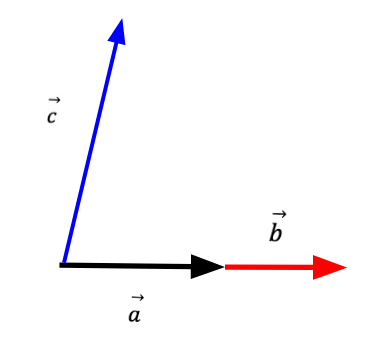
\includegraphics[height=3cm]{no-piped.png}
		\begin{center}\par\noindent Figure 4\end{center}
\end{minipage}
\newline
\newline
\par\noindent In figure 3, we see two generic vectors that are dependent \( ( \vec b = k \vec a\ )\). There is no way a parallelogram can be formed, and thus the area (or determinant) will always be zero. Likewise, in figure 4, \( \vec a \) and \( \vec b\) are still dependent. A parallelepiped cannot be formed under these circumstances and as such its volume (or determinant) will be zero.

\end{document}